\chapter{Under the Hood}
\label{how}

In this chapter we ``open the hood'', looking more closely at how some of the tools we have used --- {\tt ode45}, {\tt fzero}, and {\tt fminsearch} --- work.


\section{How ode45 Works}
\label{howode45}

According to the MATLAB documentation, {\tt ode45} uses ``an explicit Runge-Kutta formula, the Dormand-Prince pair''.  You can read about it at \emph{https://en.wikipedia.org/wiki/Runge-Kutta\_methods}, but I'll give you a sense of it here.

\index{Runge-Kutta}
\index{ode45@{\tt ode45}}
\index{Dormand-Prince}

The key idea behind all Runge-Kutta methods is to evaluate the rate function several times at each time step and use a weighted average of the computed slopes to estimate the value at the next time step.  
Different methods evaluate the rate function in different places, and compute the average with different weights.

\index{differential equation}
\index{rate function}
\index{function!rate}

As an example, I'll solve the following differential equation:

\[ \frac{dy}{dt}(t) = y \sin t \] 

Given a differential equation, it's usually straightforward to write a rate function:

\begin{code}
function res = rate_func(t, y)
    dydt = y * sin(t);
    res = dydt;
end
\end{code}

And we can call it like this:

\begin{code}
    y0 = 1;
    tspan=[0 4];
    options = odeset('Refine', 1);
    [T, Y] = ode45(@rate_func, tspan, y0, options);
\end{code}

For this example I use {\tt odeset} to set the {\tt Refine} option to 1, which tells {\tt ode45} to return only the time steps it computes, rather than interpolating between them.

\index{odeset@{\tt odeset}}

Now I can modify the rate function to plot the places where it gets evaluated:

\begin{code}
function res = rate_func(t, y)
    dydt = y * sin(t);
    res = dydt;

    plot(t, y, 'ro')
    dt = 0.01;
    ts = [t t+dt];
    ys = [y y+dydt*dt];
    plot(ts, ys, 'r-')
end
\end{code}

When \verb"rate_func" runs it plot a red circle at each location, and a short red line showing the computed slope.

\index{time step}

Figure~\ref{fig:odeplot1} shows the result.  {\tt ode45} computes 10 time steps (not counting the initial condition) and evaluates the rate function 61 times.

\begin{figure}
\centerline{\includegraphics[height=3in]{book/figs/odeplot1.eps}}
\caption{Points where {\tt ode45} evaluates the rate function.}
\label{fig:odeplot1}
\end{figure}

Figure~\ref{fig:odeplot2} shows the same plot, zoomed in on a single time step.  
The dark squares at $0.8$ to $1.2$ show the values that were returned as part of the solution.
The circles show the places where the rate function was evaluated.

We can see that {\tt ode45} evaluates the rate function several times per time step, at several places between the end points.  
We can also see that most of the places where {\tt ode45} evaluates the rate function are not part of the solution it returns, and they are not always good estimates of the solution.
This is good to know when you are writing a rate function; you should not assume that time and state you get as input variables will be part of the solution.

\begin{figure}
\centerline{\includegraphics[height=3in]{book/figs/odeplot2.eps}}
\caption{Points where {\tt ode45} evaluates the rate function, zoomed in.}
\label{fig:odeplot2}
\end{figure}

At each time step, {\tt ode45} actually computes {\em two} estimates of the next value.
By comparing them, it can estimate the magnitude of the error, which is uses to adjust the time step.
If the error is too big, it uses a smaller time step; if the error is small enough, it uses a bigger time step.
Because {\tt ode45} is \emph{adaptive} in this way, it minimizes the number of times it calls the rate function to achieve a given level of accuracy.

\index{adaptive}


\section{How fzero works}
\label{howfzero}

According to the MATLAB documentation, {\tt fzero} uses uses ``a combination of bisection, secant, and inverse quadratic interpolation methods''.

\index{fzero@{\tt fzero}}
\index{bisection}
\index{secant method}
\index{inverse quadratic interpolation
\index{root}}

To understand what that means, suppose we're trying to find a root of a function on one variable, $f(x)$, and assume we have evaluated the function at two place, $x_1$ and $x_2$, and found that the result have opposite signs.  Specifically, assume $f(x_1) > 0$ and $f(x_2) < 0$, as shown in Figure~\ref{fig:secant}.

\begin{figure}[ht]
\centerline{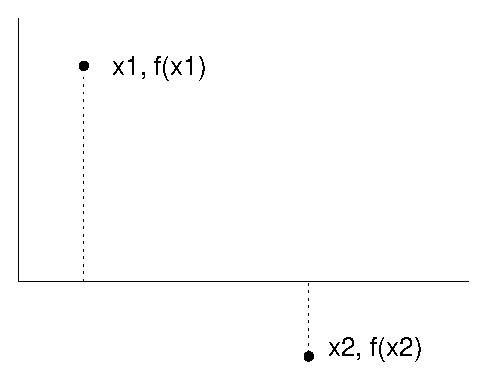
\includegraphics[height=1.6in]{book/figs/secant.eps}}
\caption{Initial state of a root-finding search.}
\label{fig:secant}
\end{figure}

As long as $f$ is continuous, there must be at least one root in this interval.  In this case we would say that $x_1$ and $x_2$
\emph{bracket} a zero.

\index{bracket}

If this was all you knew about $f$, where would you go looking for
a root?  If you said ``halfway between $x_1$ and $x_2$'',
congratulations!  You just invented a numerical method called
\emph{bisection}!

If you said, ``I would connect the dots with a straight line
and compute the zero of the line,''
congratulations!  You just invented the \emph{secant method}!

And if you said, ``I would evaluate $f$ at a third point, find the
parabola that passes through all three points, and compute the zeros
of the parabola,'' then congratulations, you just invented \emph{inverse quadratic interpolation}.

That's most of how {\tt fzero} works.  The details of how these methods are combined are interesting, but beyond the scope of this book.  You can read more at \emph{https://en.wikipedia.org/wiki/Brents\_method}.  


\section{How fminsearch works}
\label{howfminsearch}

According to the MATLAB documentation, {\tt fminsearch} uses the Nelder-Mead simplex algorithm.  You can read about it at \url{https://en.wikipedia.org/wiki/Nelder-Mead\_method}, but you might find it 
overwhelming.

\index{fminsearch@{\tt fminsearch}}
\index{Nelder-Mead}
\index{golden section search}

To give you a sense of how it works, I will present a simpler algorithm, the \emph{golden-section search}.  Suppose we're trying to find the minimum of a function of a single variable, $f(x)$.  As a starting place, assume that we have evaluated the function at three places, 
$x_1$, $x_2$, and $x_3$, and found that $x_2$ yields the lowest
value. Figure~\ref{fig:golden1} shows this initial state.

\begin{figure}[ht]
\centerline{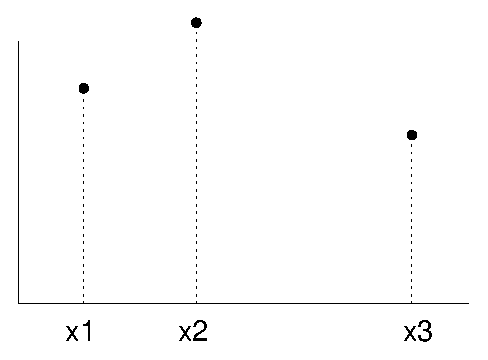
\includegraphics[height=1.5in]{book/figs/golden1.eps}}
\caption{Initial state of a golden-section search.}
\label{fig:golden1}
\end{figure}

If $f$ is continuous, there has to be at least one
minimum point between $x_1$ and $x_3$.

\index{minimum}

The next step is to choose a fourth point, $x_4$, and evaluate
$f(x_4)$.  There are two possible outcomes, depending on whether
$f(x_4)$ is greater than $f(x_2)$.
Figure~\ref{fig:golden2} shows the two possible states.

\begin{figure}[ht]
\centerline{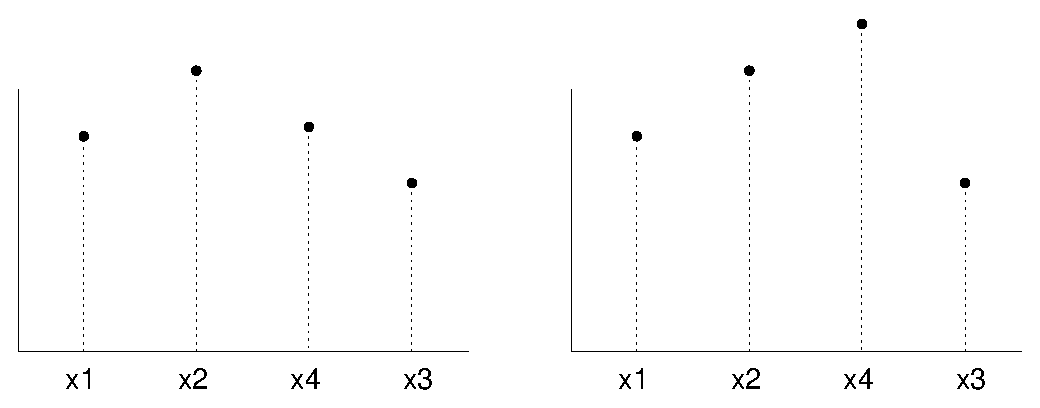
\includegraphics[height=1.5in]{book/figs/golden2.eps}}
\caption{Possible states of a golden-section search after evaluating $f(x_4)$.}
\label{fig:golden2}
\end{figure}

If $f(x_4)$ is less than than $f(x_2)$ (shown on the left), the
local minimum must be between $x_2$ and $x_3$, so we would discard $x_1$ and proceed with the new triple $(x_2, x_4, x_3)$.

If $f(x_4)$ is greater than $f(x_2)$ (shown on the right), the
local minimum must be between $x_1$ and $x_4$, so we would discard $x_3$ and proceed with the new triple $(x_1, x_2, x_4)$.

Either way the range gets smaller and our estimate of the optimal value of $x$ gets better.

This method works for almost any value of $x_4$, but some choices
are better than others.  You might be tempted to bisect the interval between $x_2$ and $x_3$, but that turns out not to be the best choice.  You can read about a better option at \emph{https://en.wikipedia.org/wiki/Golden-section\_search\#Probe\_point\_selection}.
